\section{Proofs of the exact moment results}
\label{app:proofs}

\subsection*{Proposition~\ref{prop:mean}}
\begin{proof}
  Condition on $r_j$. The other $G-1$ rewards are i.i.d.\ Bernoulli$(p)$ and, given $r_j$, are
  independent of $\score(y_j)$, so
  $\E[w(k, r_j)\score(y_j)] = \sum_{r} \Pr[r]\, W_r\, u_r$. Summing over $j$ and applying
  \eqref{eq:score-identity} gives $\E[z] = p\,(W_1 - W_0)\,u_1 = \lambda h$.
\end{proof}

\subsection*{Proposition~\ref{prop:cov}}
\begin{proof}
  Split $\E[z z^{\!\top}]$ into diagonal and off-diagonal terms. The diagonal contributes
  $G^{-1}[p Q_1 M_1 + (1-p) Q_0 M_0]$ with $M_r = S_r + u_r u_r^{\!\top}$. For $j \neq l$,
  condition on $(r_j, r_l)$ and on the count $m'$ among the remaining $G-2$ responses; the two
  scores are then conditionally independent, giving
  $\frac{G-1}{G}\sum_{a,b}\Pr[a]\Pr[b]\,C_{ab}\,u_a u_b^{\!\top}$, which collapses to
  $\frac{G-1}{G} p^2 (C_{11} - 2C_{10} + C_{00}) U$ by \eqref{eq:score-identity}. Subtracting
  $\E[z]\E[z]^{\!\top} = \lambda^2 p^2 U$ completes the proof.
\end{proof}

\section{Reproducing the results}
\label{app:repro}

Every figure and table is regenerated from stored run records by
\texttt{analysis/figures.py} and \texttt{analysis/tables.py}; no number in this paper is
transcribed by hand. Each run writes a manifest holding the configuration, its hash, the commit the
code was at, and the interpreter and platform it ran on.

The exactness tests in \texttt{tests/} check every analytic result in Section~\ref{sec:theory}
against brute-force enumeration, and check the batched estimator against the reference
implementation term by term.

\section{The estimator family as a table}
\label{app:family}

Because the advantage depends only on $(k, r)$, an estimator is a $(G+1) \times 2$ array, and the
moments in \eqref{eq:contractions} are contractions of that array against a binomial distribution.
This is what makes the exact treatment cheap: no sampling is involved in evaluating
$\lambda(p, G)$, $Q_r$ or $C_{ab}$ for any member of the family, at any group size.


\section{Noise terms across task families}
\label{app:cross-family}

The corollary relating within-prompt noise to the reward histogram assumes a shared score
scale, which holds within a task family and not between families of different answer shape.
The measurements below make the size of that effect explicit.

\begin{table}[t]
  \centering
  \small
  \begin{tabular}{lcccccc}
\toprule
corpus & pass rate & $\E[p(1-p)]$ & $\tau_b$ & $\tau_w$ & $G^{\star}$ & $\tau_w/\E[p(1-p)]$ \\
\midrule
count letter & 0.280 & 0.178 & 4.35e+02 & 1.16e+04 & 6.15 & 0.27 \\
nth word & 0.326 & 0.138 & 4.88e+03 & 2.01e+04 & 3.03 & 0.61 \\
add two & 0.546 & 0.062 & 1.29e+04 & 3.55e+04 & 2.66 & 2.40 \\
mixed & 0.193 & 0.071 & 4.31e+03 & 1.20e+04 & 2.67 & 0.71 \\
\bottomrule
\end{tabular}
  \caption{Noise terms measured on a pretrained model. The last column would be constant if the
  score scale were shared across families; it is not, and it is not meant to be.}
  \label{tab:real}
\end{table}

\begin{figure}[t]
  \centering
  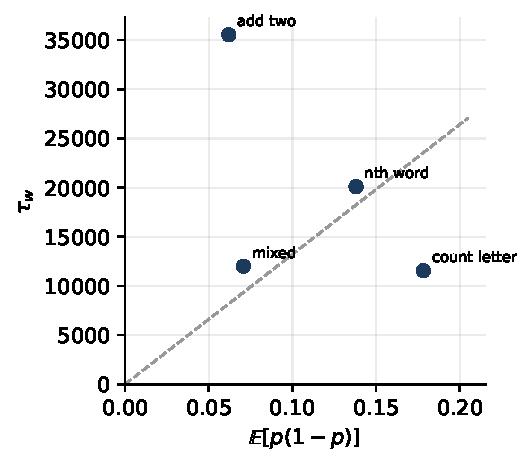
\includegraphics[width=0.95\linewidth]{figures/real_model.pdf}
  \caption{Within-prompt noise against the reward histogram across corpora, with a single fitted
  scale. The scatter is the score scale differing between task families.}
  \label{fig:real-model}
\end{figure}
